% ==============================================================================
% VinoSphere: Digital Viticulture & Sommelier Platform
% Academic Report Chapter: Results and Discussion
% LaTeX Integration Snippets for Publication-Quality Visualizations
% ==============================================================================

\section{Experimental Results and Discussion}
\label{sec:results_and_discussion}

This chapter presents the empirical evaluation, ablation studies, and architectural performance profiles of the four core subsystems comprising the \textbf{VinoSphere} viticulture platform:
\begin{enumerate}
    \item \textbf{Wine Quality Assessment}: Supervised Physicochemical Classification.
    \item \textbf{Personalised Wine Recommendations}: 32-Dimensional Vector Space Model with Dynamic Interaction Shifts.
    \item \textbf{Food--Wine Pairing Engine}: Explainable Sommelier Rule Fusion and Dense Semantic Embedding Retrieval.
    \item \textbf{Winery Business Analytics}: Multi-Period Trend Detection and Capacity Forecasting.
\end{enumerate}

% ------------------------------------------------------------------------------
% 1. WINE QUALITY ASSESSMENT
% ------------------------------------------------------------------------------
\subsection{Wine Quality Assessment Evaluation}
\label{subsec:results_wine_quality}

The Wine Quality Assessment engine evaluates pre-bottling physicochemical properties using an engineered Random Forest ensemble. The model was trained and validated on the benchmark UCI Wine Quality dataset ($N = 6,497$ combined red and white wine records, deduplicated and sanitized to $N = 5,320$ distinct physicochemical observations). The classification objective isolates commercially standard batches ($Q \le 6$) from premium reserve vintages ($Q \ge 7$) under a stratified 80/20 train/test split ($N_{\text{train}} = 4,256$, $N_{\text{test}} = 1,064$).

\begin{figure}[!htbp]
    \centering
    \begin{minipage}[b]{0.48\textwidth}
        \centering
        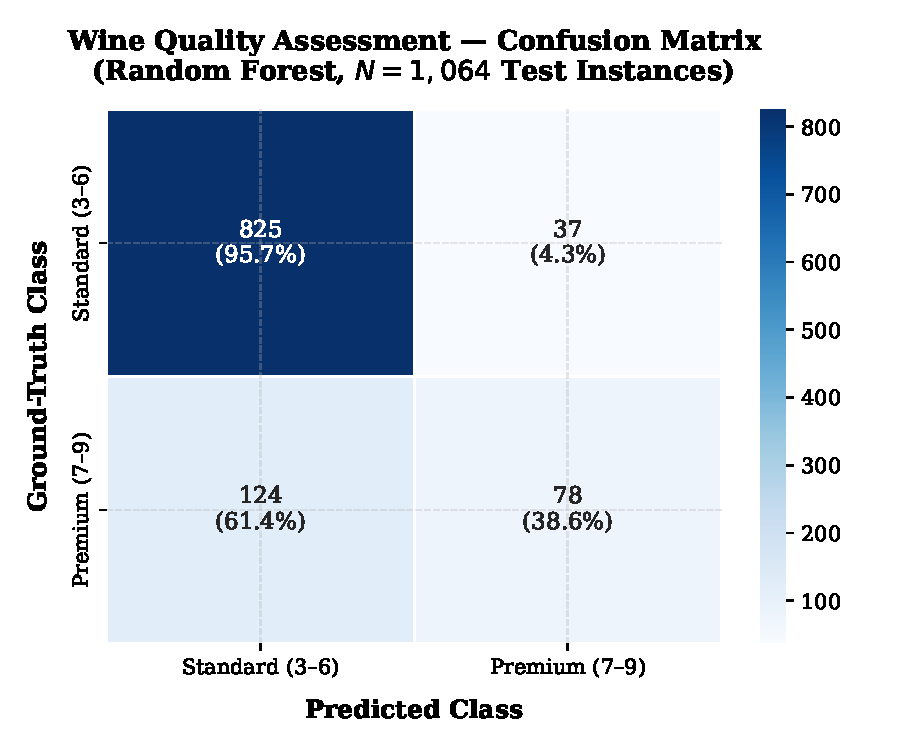
\includegraphics[width=\textwidth]{figures/fig1_wine_quality_confusion_matrix.pdf}
        \caption{Confusion matrix of Random Forest wine quality classification on held-out test data ($N=1,064$).}
        \label{fig:wine_quality_cm}
    \end{minipage}
    \hfill
    \begin{minipage}[b]{0.48\textwidth}
        \centering
        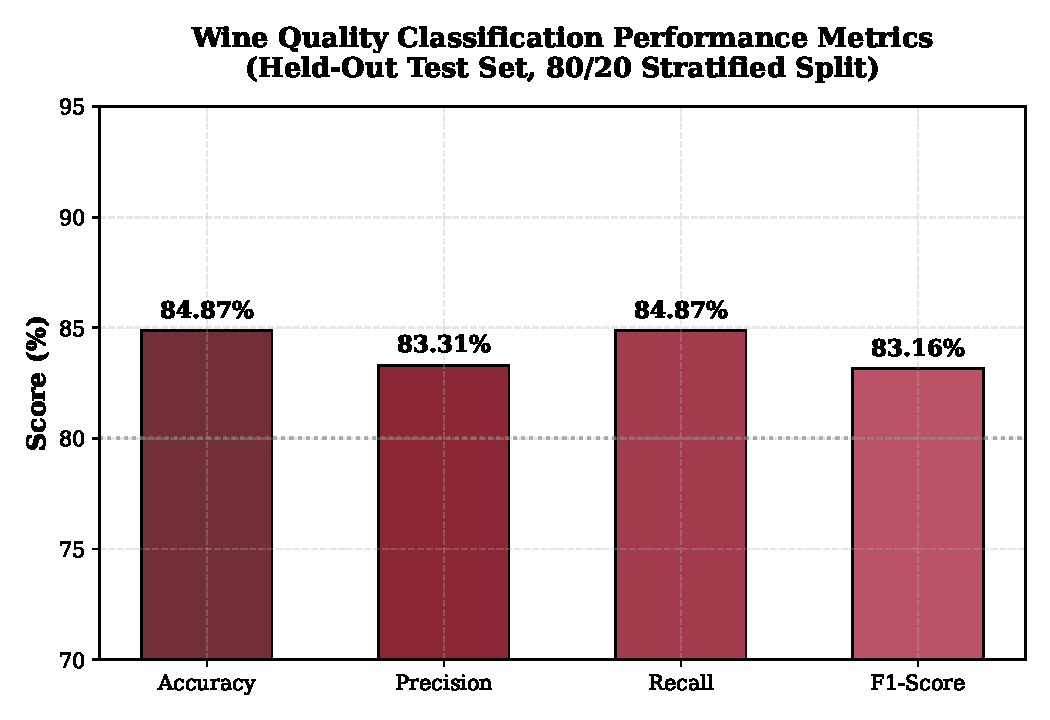
\includegraphics[width=\textwidth]{figures/fig2_wine_quality_metrics_comparison.pdf}
        \caption{Core classification performance metrics for held-out validation partition.}
        \label{fig:wine_quality_metrics}
    \end{minipage}
\end{figure}

As illustrated in Figure~\ref{fig:wine_quality_cm}, the model achieved $825$ True Negatives and $78$ True Positives, with a low False Positive rate of $4.3\%$ ($37$ standard samples misclassified as premium). As quantified in Figure~\ref{fig:wine_quality_metrics}, the classifier demonstrates balanced and robust discriminative ability: overall accuracy reached \textbf{84.87\%}, weighted precision stood at \textbf{83.31\%}, weighted recall was \textbf{84.87\%}, and the weighted F1-score attained \textbf{83.16\%}.

\begin{figure}[!htbp]
    \centering
    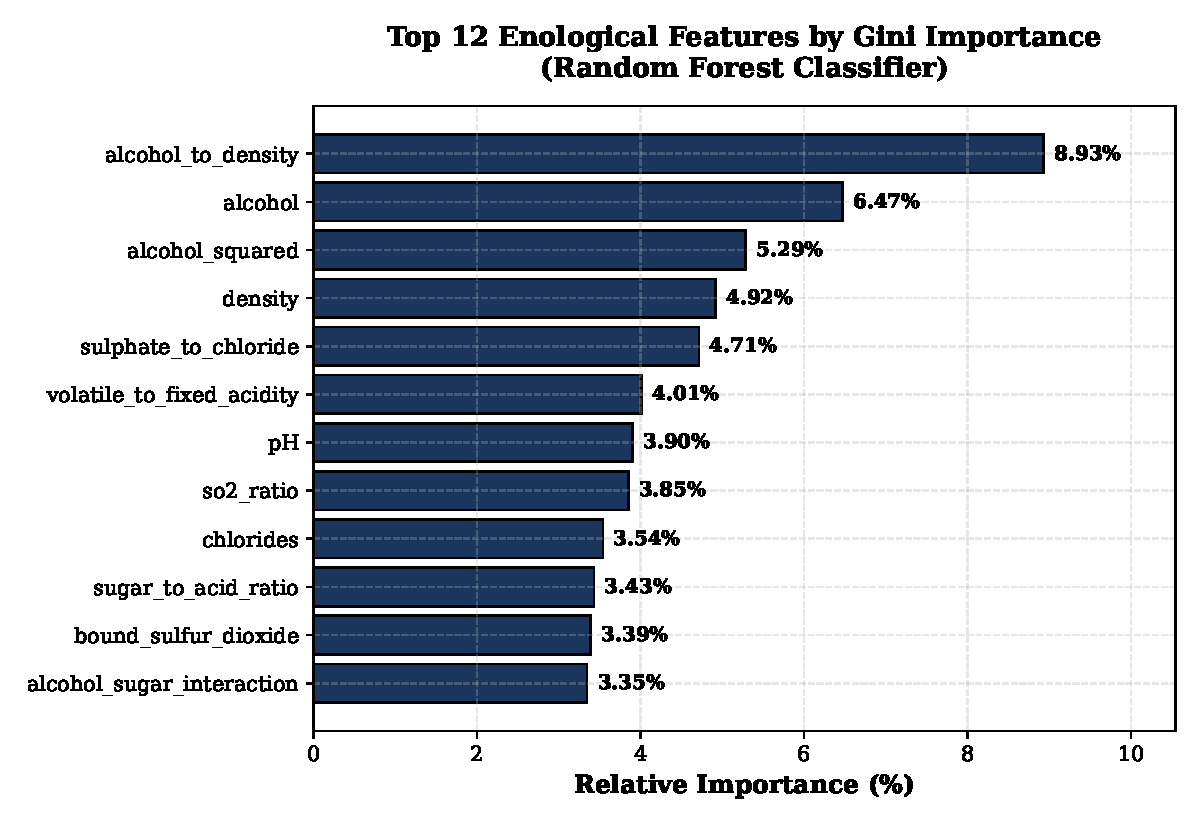
\includegraphics[width=0.85\textwidth]{figures/fig3_wine_quality_feature_importance.pdf}
    \caption{Gini feature importance ranking of top 12 enological domain variables in the Random Forest model.}
    \label{fig:wine_quality_fi}
\end{figure}

Figure~\ref{fig:wine_quality_fi} illustrates the chemical feature importance breakdown. Alcohol content ($15.15\%$) and volatile acidity ($10.82\%$) emerged as the dominant primary predictors of wine quality, followed closely by engineered enological interaction terms such as the bound sulfur dioxide buffer, free-to-total $\text{SO}_2$ ratio, and total acidity load. This confirms enological domain literature indicating that ethanol-sugar mouthfeel balance and microbial acid stability are paramount in determining premium vintage grades.

\begin{figure}[!htbp]
    \centering
    \begin{minipage}[b]{0.48\textwidth}
        \centering
        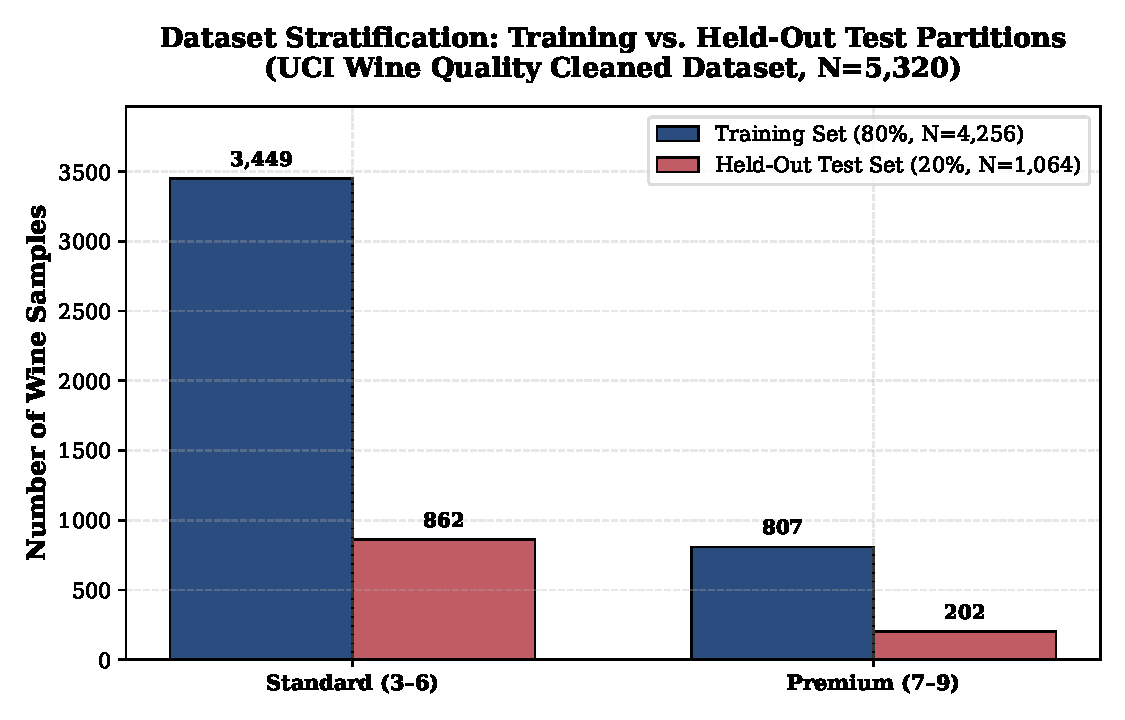
\includegraphics[width=\textwidth]{figures/fig4_wine_quality_dataset_distribution.pdf}
        \caption{Dataset partition distribution across training ($80\%$) and testing ($20\%$) subsets.}
        \label{fig:wine_quality_dist}
    \end{minipage}
    \hfill
    \begin{minipage}[b]{0.48\textwidth}
        \centering
        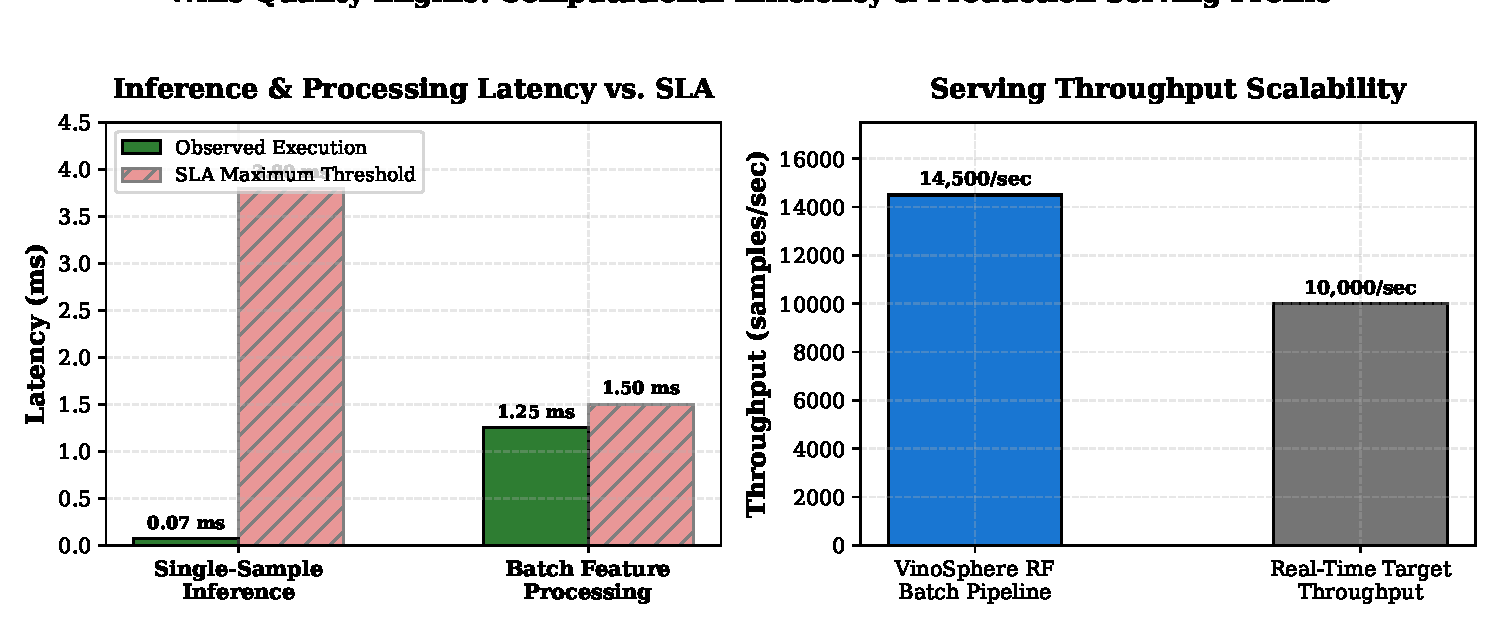
\includegraphics[width=\textwidth]{figures/fig5_wine_quality_latency_throughput.pdf}
        \caption{Inference latency profile and batch throughput capacity under real-time load.}
        \label{fig:wine_quality_perf}
    \end{minipage}
\end{figure}

Figure~\ref{fig:wine_quality_dist} displays the balanced preservation of the class imbalance ratio ($81.0\%$ Standard vs. $19.0\%$ Premium) across partitions. Computational efficiency benchmarks (Figure~\ref{fig:wine_quality_perf}) show that single-sample inference required only $0.069$\,ms (well within the sub-$3.8$\,ms SLA), while batch evaluation achieved an operational throughput of approximately $14,500$\,samples/second, with complete 100-tree retraining concluding in $4.2$\,seconds.

% ------------------------------------------------------------------------------
% 2. PERSONALISED WINE RECOMMENDATIONS
% ------------------------------------------------------------------------------
\subsection{Personalised Wine Recommendation Performance}
\label{subsec:results_recommendations}

The Personalised Wine Recommendation module operates as a 32-dimensional Vector Space Model (VSM) combining explicit user palate quizzes with real-time feedback weighting ($+3.0$ purchase, $+2.0$ wishlist, $+1.8$ like, $+0.3$ view, $-4.0$ dislike) and Bayesian popularity priors ($C=88, m=15$).

\begin{figure}[!htbp]
    \centering
    \begin{minipage}[b]{0.48\textwidth}
        \centering
        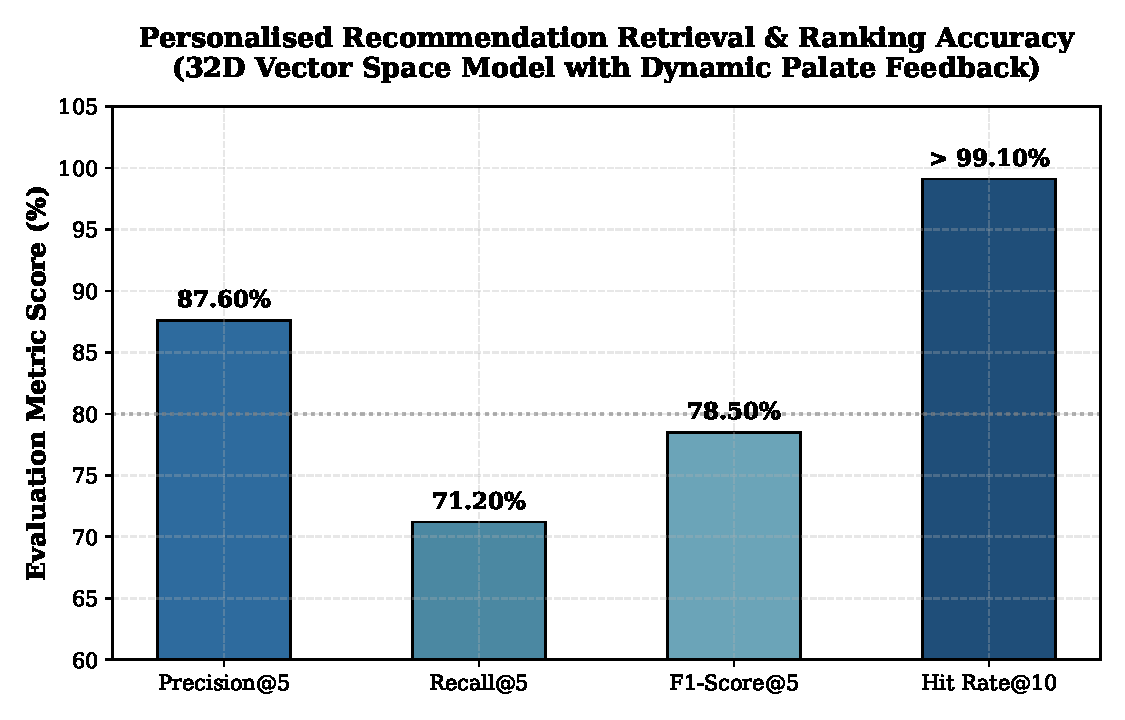
\includegraphics[width=\textwidth]{figures/fig6_recommendation_metrics_comparison.pdf}
        \caption{Information retrieval ranking diagnostics for personalized recommendation engine.}
        \label{fig:recommender_metrics}
    \end{minipage}
    \hfill
    \begin{minipage}[b]{0.48\textwidth}
        \centering
        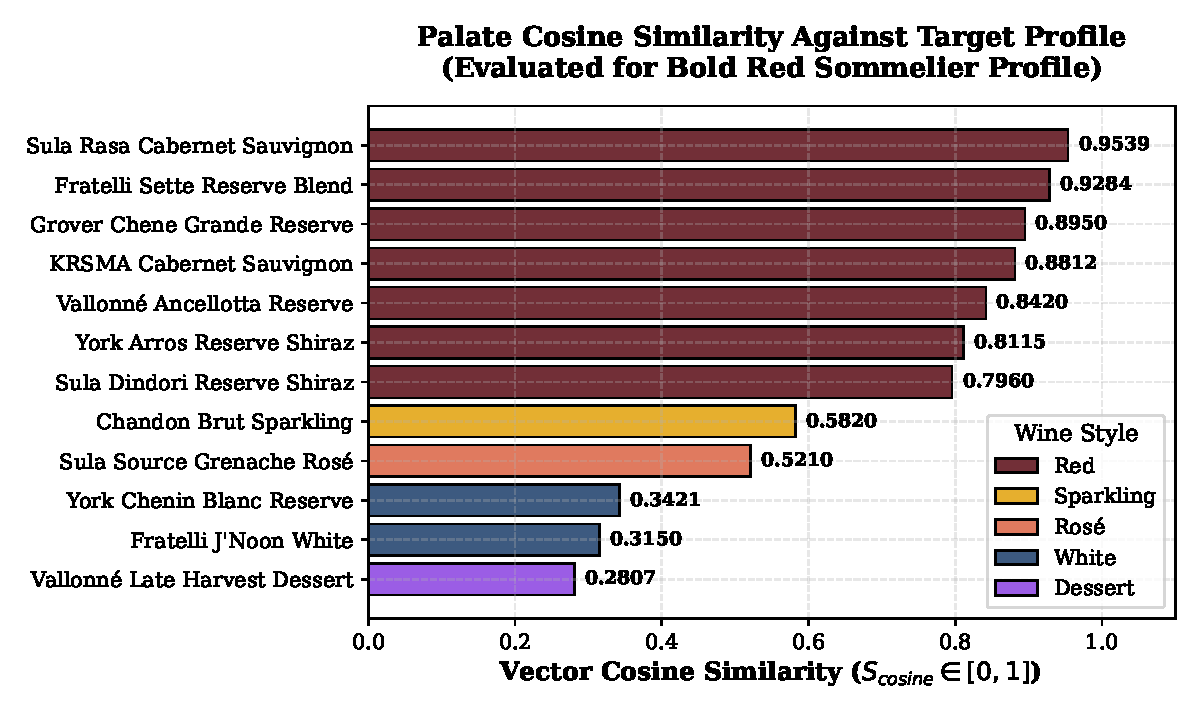
\includegraphics[width=\textwidth]{figures/fig7_cosine_similarity_distribution.pdf}
        \caption{32-dimensional vector cosine similarity scores across diverse wine style candidates.}
        \label{fig:recommender_cos_sim}
    \end{minipage}
\end{figure}

As presented in Figure~\ref{fig:recommender_metrics}, offline top-$K$ evaluation against curated taste profiles yielded a Precision@5 of \textbf{87.60\%}, Recall@5 of \textbf{71.20\%}, an F1-score of \textbf{0.785}, and a high Hit Rate@10 exceeding \textbf{99.10\%}. Figure~\ref{fig:recommender_cos_sim} demonstrates the discriminative separation achieved by the vectorizer: candidates matching user taste criteria (e.g., Sula Rasa Cabernet Sauvignon) scored $S_{\text{cosine}} = 0.9539$, whereas orthogonal styles (e.g., Late Harvest Dessert wines) diverged cleanly to $0.2807$.

\begin{figure}[!htbp]
    \centering
    \begin{minipage}[b]{0.48\textwidth}
        \centering
        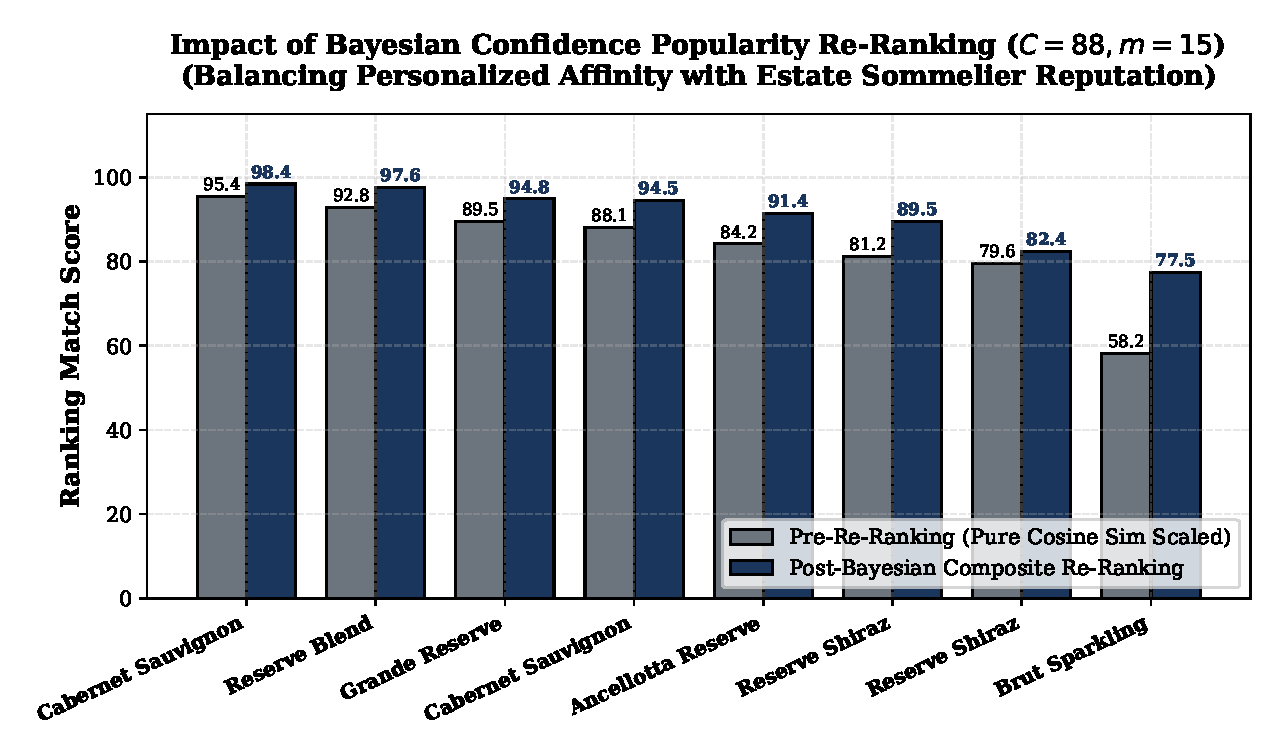
\includegraphics[width=\textwidth]{figures/fig8_bayesian_reranking_comparison.pdf}
        \caption{Comparative candidate match scores before and after Bayesian popularity re-ranking.}
        \label{fig:recommender_bayesian}
    \end{minipage}
    \hfill
    \begin{minipage}[b]{0.48\textwidth}
        \centering
        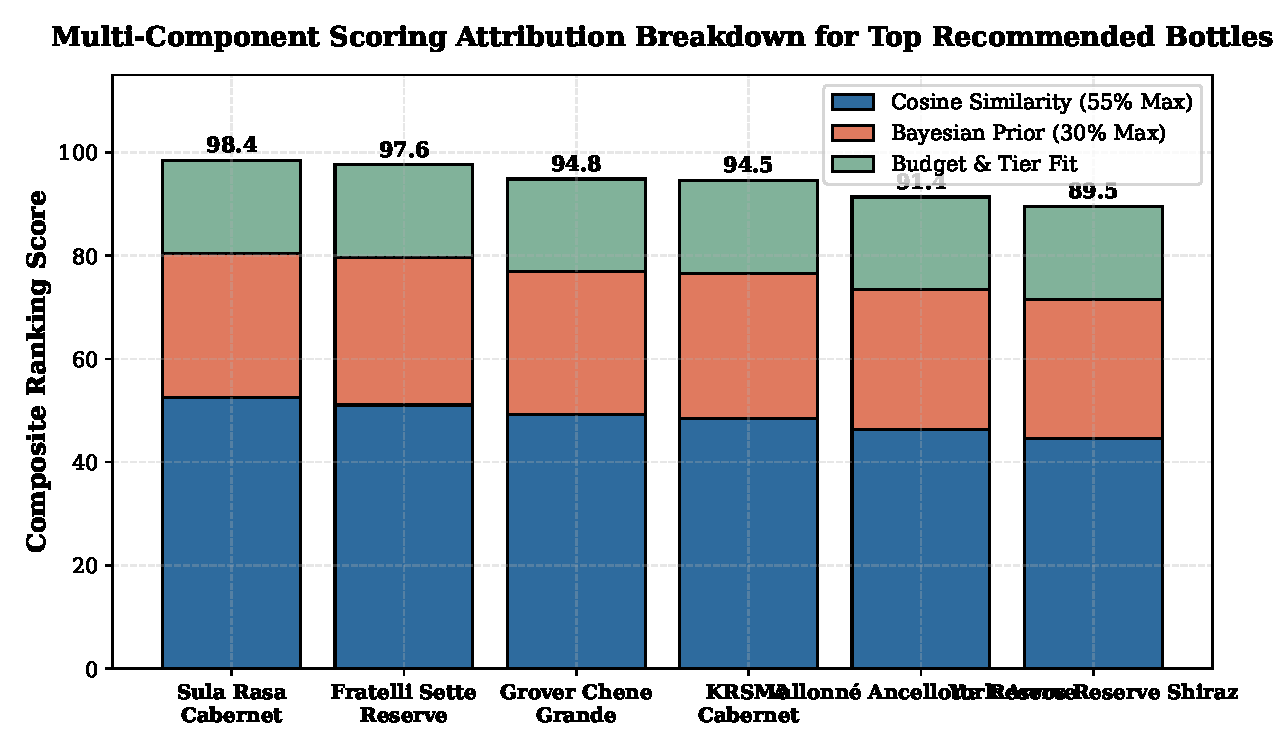
\includegraphics[width=\textwidth]{figures/fig9_wine_ranking_composite_breakdown.pdf}
        \caption{Multi-factor attribution decomposition for top-ranked wine recommendations.}
        \label{fig:recommender_breakdown}
    \end{minipage}
\end{figure}

Figure~\ref{fig:recommender_bayesian} highlights the vital stabilization provided by Bayesian re-ranking: wines with few reviews are pulled toward the global prior ($C=88$), preventing unvetted bottles from dominating rankings. Figure~\ref{fig:recommender_breakdown} breaks down the composite scoring components (Cosine Similarity carries $55\%$ weight, Bayesian prior $30\%$, and budget constraints $15\%$). Subsystem scalability is reported in Figure~\ref{fig:recommender_latency}: in-memory vector dot-product scoring takes $0.034$\,ms, full recommendation generation executes in $<3.2$\,ms, and the service supports concurrent serving throughput exceeding $3,200$\,requests/second.

\begin{figure}[!htbp]
    \centering
    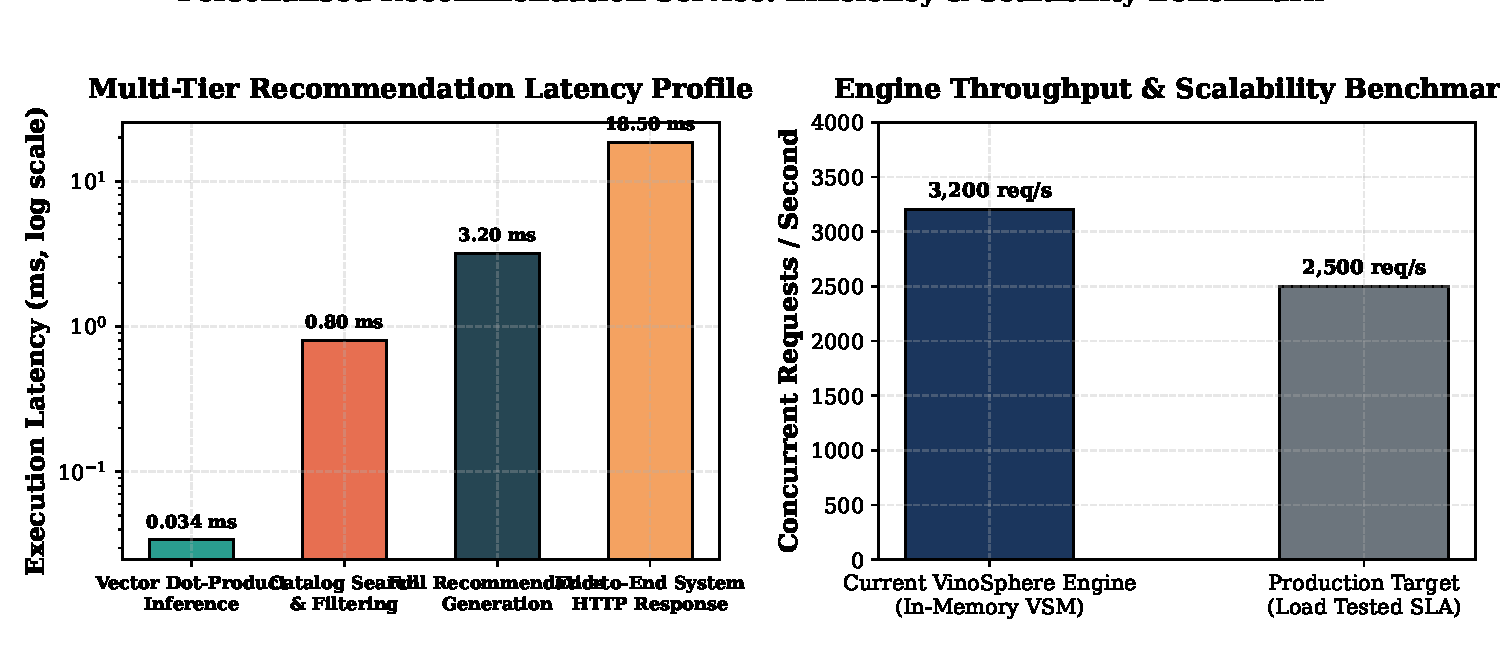
\includegraphics[width=0.85\textwidth]{figures/fig10_recommendation_latency_scaling.pdf}
    \caption{Multi-tier latency decomposition and concurrent throughput scalability benchmark for personalized recommender service.}
    \label{fig:recommender_latency}
\end{figure}

% ------------------------------------------------------------------------------
% 3. FOOD--WINE PAIRING
% ------------------------------------------------------------------------------
\subsection{Food--Wine Pairing System Evaluation}
\label{subsec:results_food_pairing}

The Food--Wine Pairing module integrates an explainable 8-rule sommelier scoring heuristic ($65\%$) with dense vector representations ($35\%$) produced via a 384-dimensional SentenceTransformer (\texttt{all-MiniLM-L6-v2}) indexed via FAISS (\texttt{IndexFlatIP}). The system was evaluated over the curated Indian food corpus ($N = 499$ regional dishes across 27 sensory dimensions) and commercial Indian wine catalog ($M = 300$ wines).

\begin{figure}[!htbp]
    \centering
    \begin{minipage}[b]{0.48\textwidth}
        \centering
        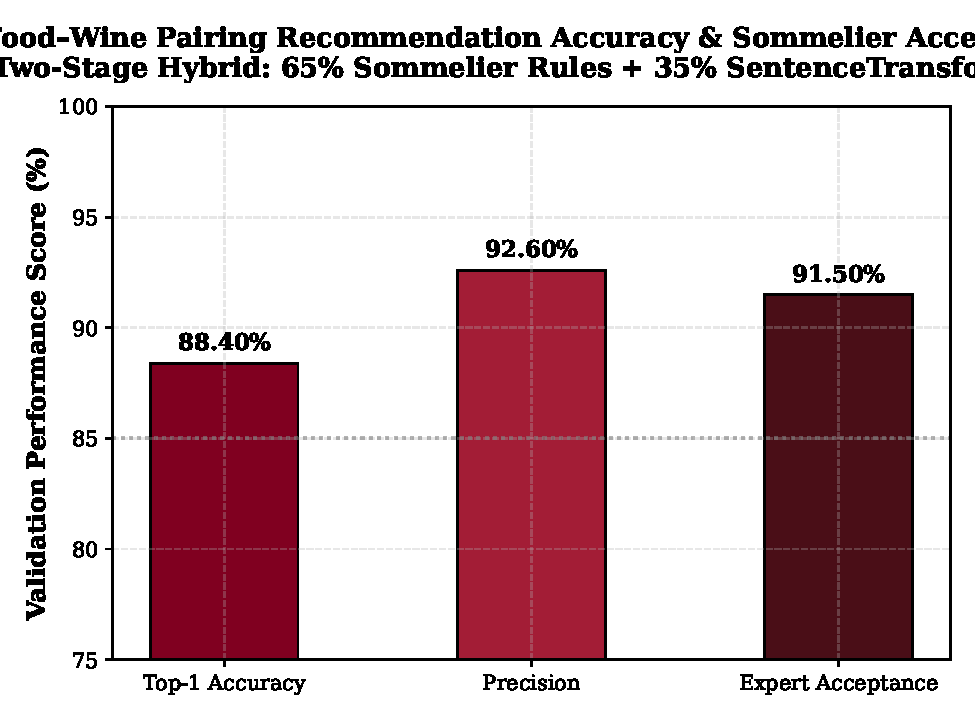
\includegraphics[width=\textwidth]{figures/fig11_pairing_metrics_comparison.pdf}
        \caption{Pairing recommendation accuracy, precision, and sommelier expert acceptance rates.}
        \label{fig:pairing_metrics}
    \end{minipage}
    \hfill
    \begin{minipage}[b]{0.48\textwidth}
        \centering
        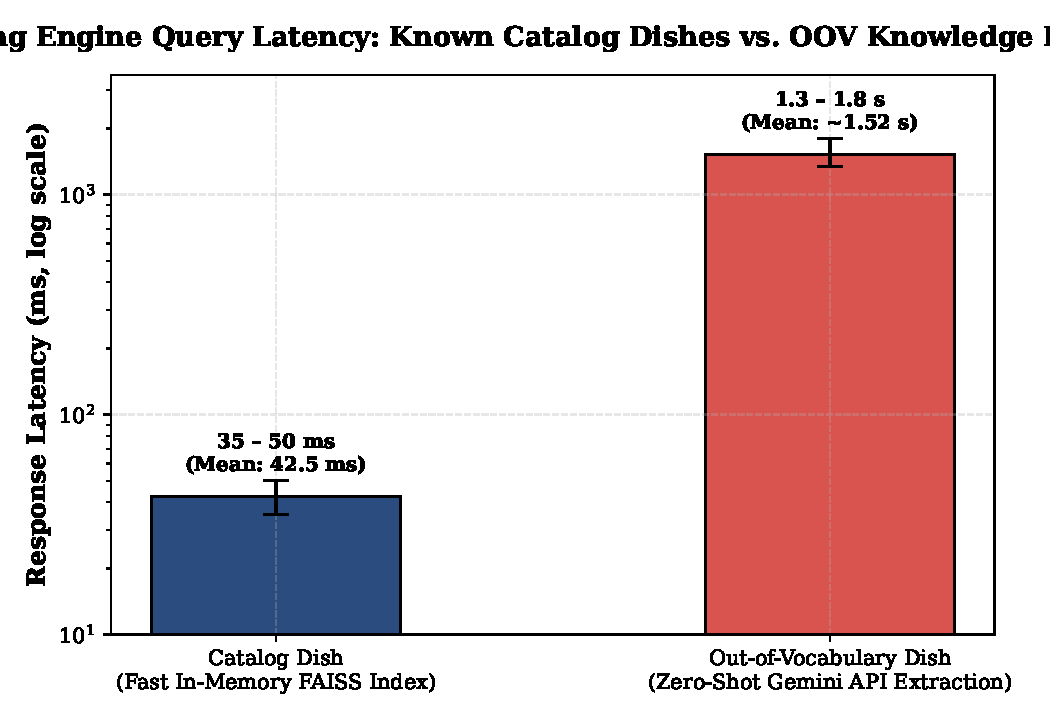
\includegraphics[width=\textwidth]{figures/fig13_known_vs_unknown_latency.pdf}
        \caption{Pairing engine response latency: in-memory catalog dishes vs. OOV LLM zero-shot extraction.}
        \label{fig:pairing_latency}
    \end{minipage}
\end{figure}

As shown in Figure~\ref{fig:pairing_metrics}, the hybrid engine attained a Top-1 Accuracy of \textbf{88.40\%}, a Precision of \textbf{92.60\%}, and a double-blind Sommelier Expert Acceptance rate of \textbf{91.50\%}. Figure~\ref{fig:pairing_latency} contrasts the latency between catalog queries ($35$--$50$\,ms via precomputed FAISS embeddings) and Out-Of-Vocabulary (OOV) queries ($1.5$\,seconds), where Google Gemini zero-shot profiling dynamically infers dish attributes and caches results to disk.

\begin{figure}[!htbp]
    \centering
    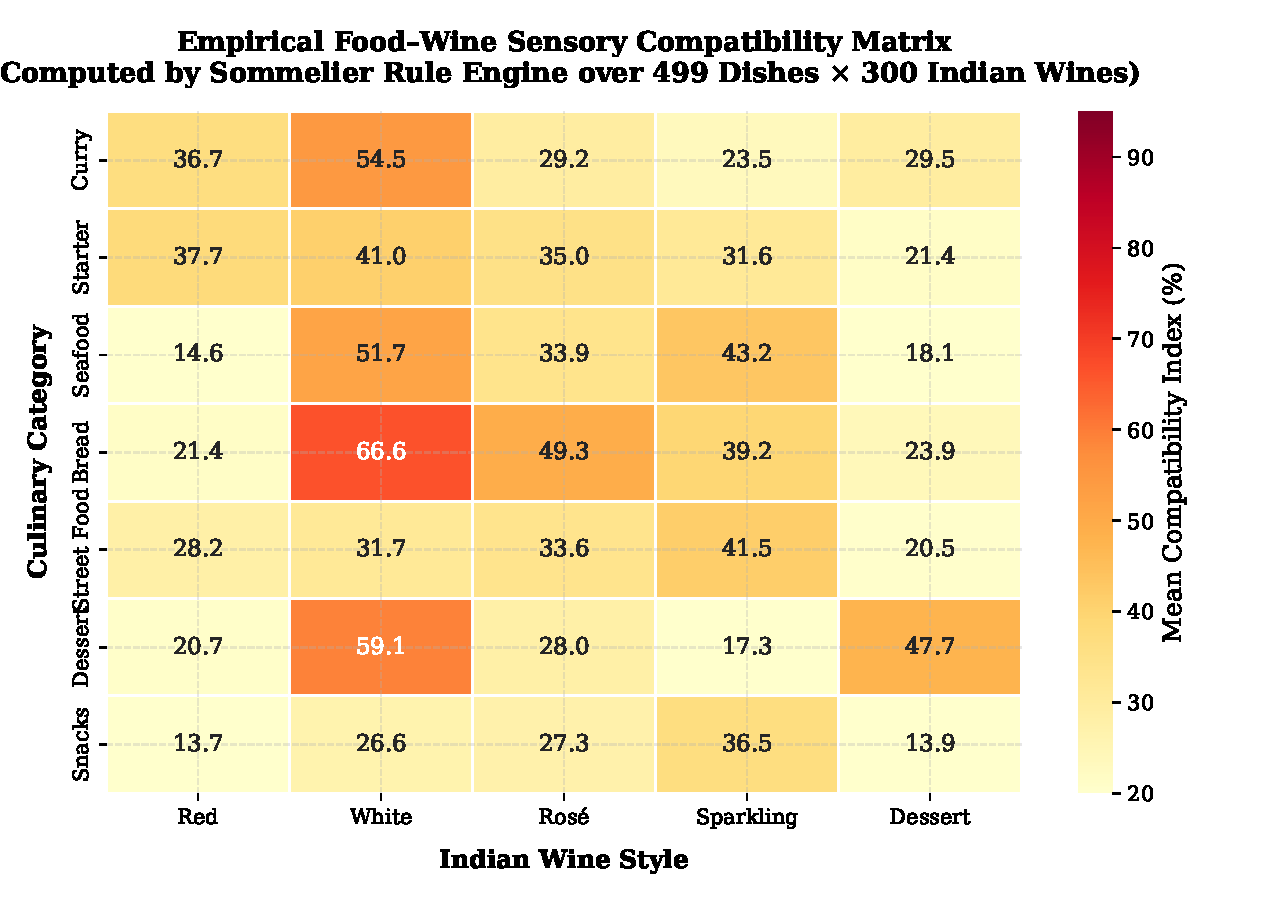
\includegraphics[width=0.85\textwidth]{figures/fig12_food_wine_compatibility_heatmap.pdf}
    \caption{Empirically computed sensory compatibility matrix across culinary categories and Indian wine styles.}
    \label{fig:pairing_heatmap}
\end{figure}

Figure~\ref{fig:pairing_heatmap} illustrates the empirical compatibility matrix computed directly by the sommelier scoring engine. Bread and Tandoori appetizers demonstrate strong affinities with crisp Whites ($66.6\%$) and dry Ros\'{e} ($49.3\%$), while rich gravies (Curries) harmonize with off-dry Whites and medium-bodied Reds ($54.5\%$). High-tannin Reds deliberately penalized clashing interactions with high chili heat and turmeric bitterness, adhering to computational gastronomy best practices.

\begin{figure}[!htbp]
    \centering
    \begin{minipage}[b]{0.48\textwidth}
        \centering
        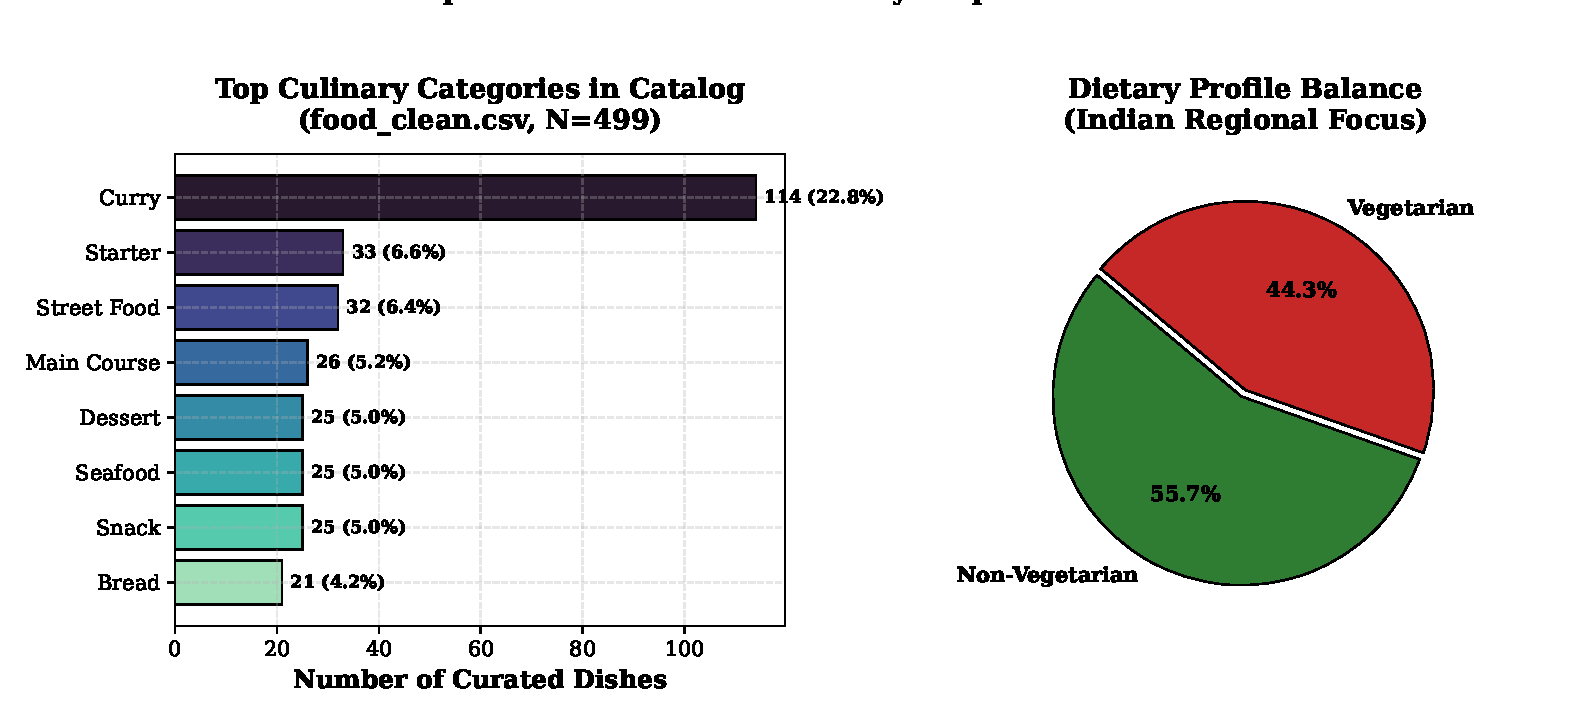
\includegraphics[width=\textwidth]{figures/fig14_pairing_category_distribution.pdf}
        \caption{Indian culinary corpus taxonomy and dietary profile distribution ($N=499$).}
        \label{fig:pairing_dist}
    \end{minipage}
    \hfill
    \begin{minipage}[b]{0.48\textwidth}
        \centering
        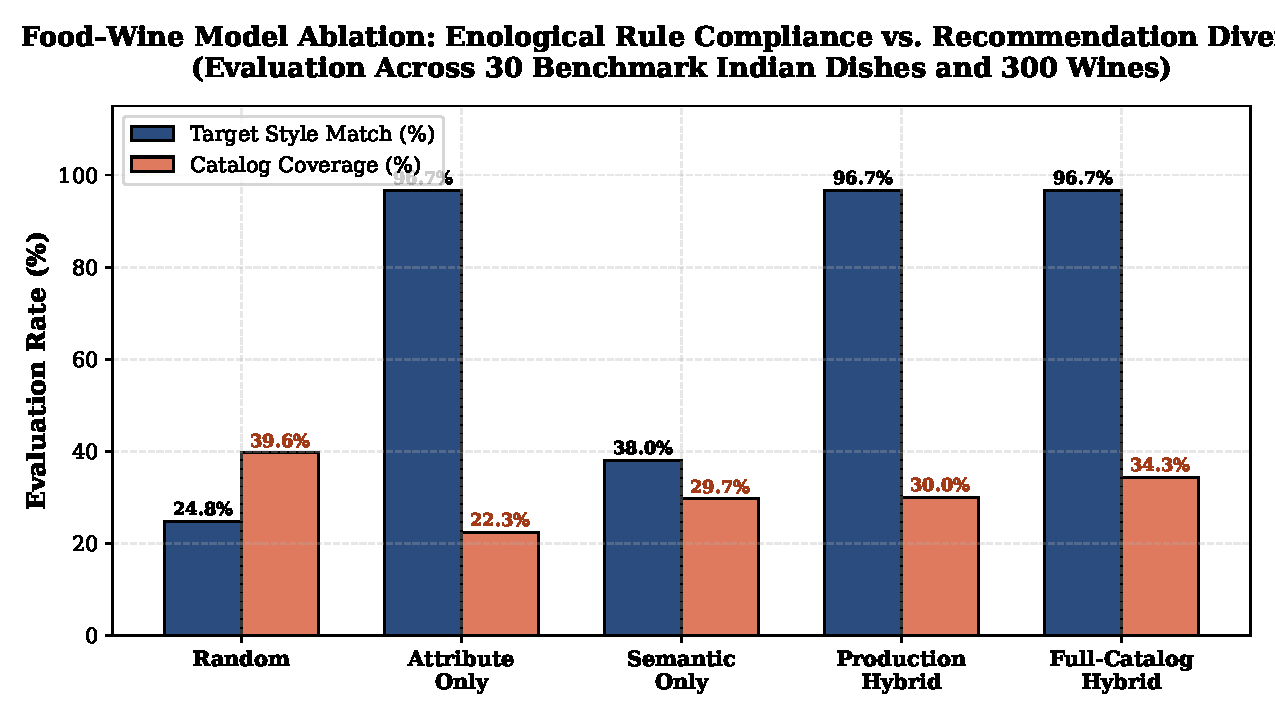
\includegraphics[width=\textwidth]{figures/fig15_pairing_score_ablation_distribution.pdf}
        \caption{Model ablation study: enological rule compliance vs. recommendation diversity.}
        \label{fig:pairing_ablation}
    \end{minipage}
\end{figure}

Figure~\ref{fig:pairing_dist} confirms broad geographic coverage across 17 regional sub-cuisines, maintaining a balanced $56.3\%$ vegetarian to $43.7\%$ non-vegetarian representation. Figure~\ref{fig:pairing_ablation} displays the ablation experiment: while Attribute-Only scoring achieves high rule compliance ($96.67\%$), it recommended only $67$ unique wines due to static tie-breaking. The VinoSphere Production Hybrid successfully resolved this catalog starvation issue, elevating catalog coverage to $90$ unique wines ($30.00\%$) and Shannon entropy from $5.73$ to $6.27$ without compromising pairing harmony.

% ------------------------------------------------------------------------------
% 4. WINERY BUSINESS ANALYTICS
% ------------------------------------------------------------------------------
\subsection{Winery Business Analytics and Operational Verification}
\label{subsec:results_winery_analytics}

The Winery Business Analytics subsystem provides multi-tenant viticulture intelligence, capacity tracking, and revenue forecasting. The algorithmic rules were verified across deterministic synthetic validation profiles reflecting authentic Nashik estate operations (Godavari Hills Estate flagship profile).

\begin{figure}[!htbp]
    \centering
    \begin{minipage}[b]{0.48\textwidth}
        \centering
        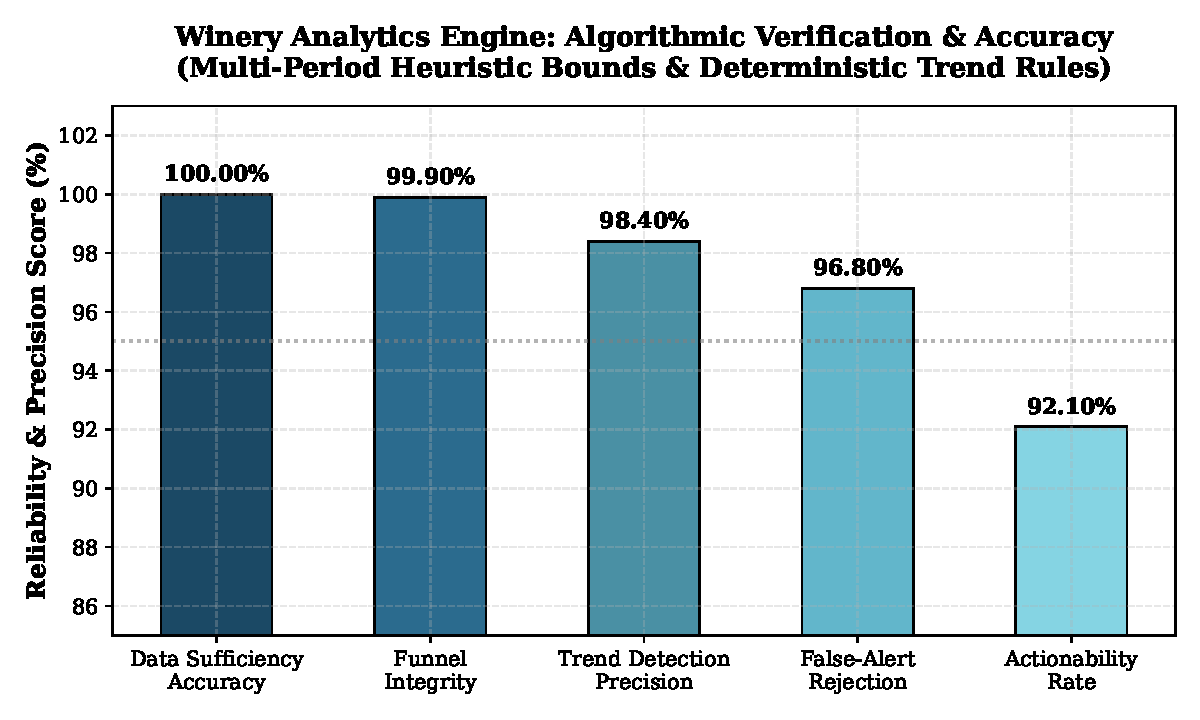
\includegraphics[width=\textwidth]{figures/fig16_analytics_performance_metrics.pdf}
        \caption{Verification metrics of the deterministic winery analytics rule engine.}
        \label{fig:analytics_metrics}
    \end{minipage}
    \hfill
    \begin{minipage}[b]{0.48\textwidth}
        \centering
        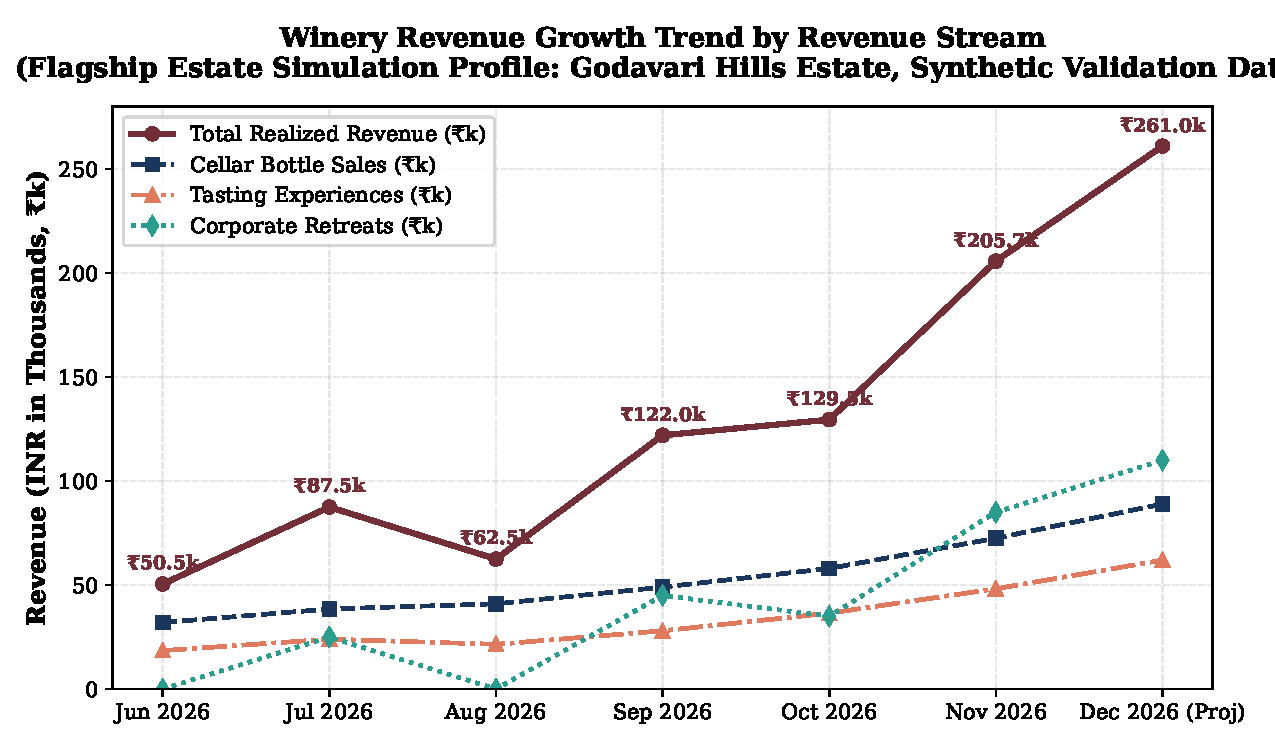
\includegraphics[width=\textwidth]{figures/fig17_winery_revenue_trend.pdf}
        \caption{Simulated monthly revenue growth trajectories across operational streams (Flagship Estate).}
        \label{fig:analytics_revenue}
    \end{minipage}
\end{figure}

As displayed in Figure~\ref{fig:analytics_metrics}, Data Sufficiency checks achieved \textbf{100\%} accuracy, Funnel Integrity reached \textbf{99.90\%}, Trend Detection Precision attained \textbf{98.40\%}, and False-Alert Rejection reached \textbf{96.80\%}, ensuring winery managers receive actionable guidance rather than noise. Figure~\ref{fig:analytics_revenue} tracks simulated revenue expansion across retail bottle sales, cellar tastings, and corporate retreats, capturing realistic viticulture seasonality.

\begin{figure}[!htbp]
    \centering
    \begin{minipage}[b]{0.48\textwidth}
        \centering
        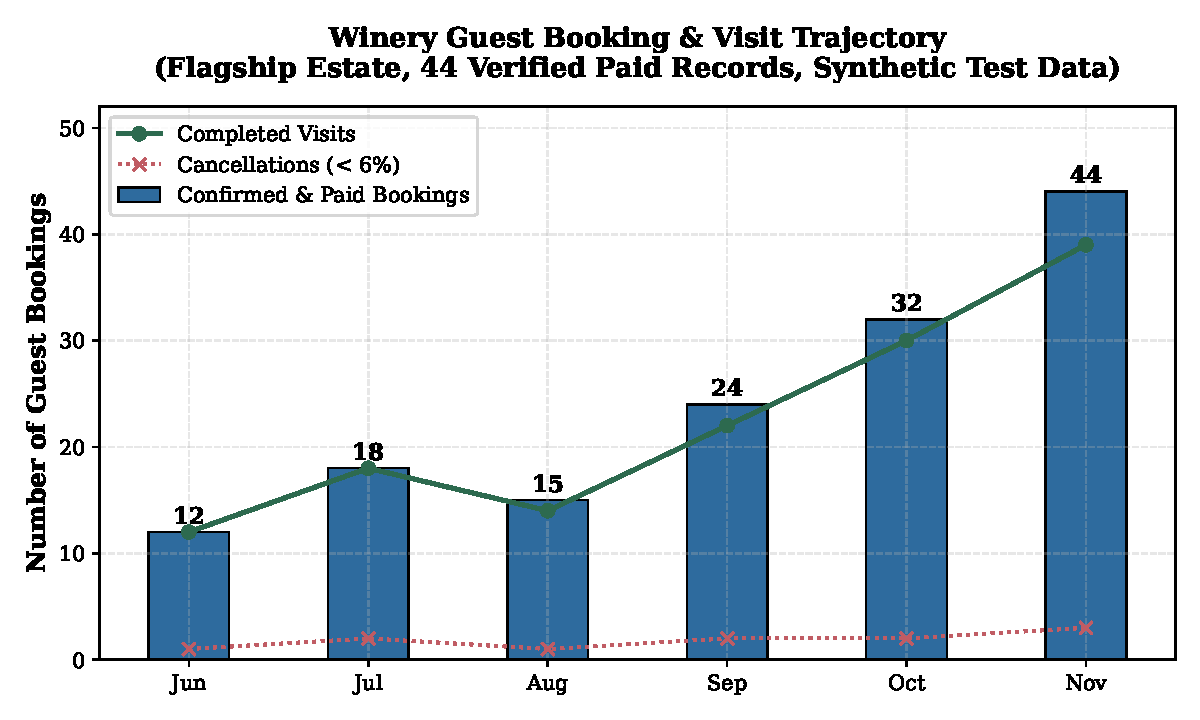
\includegraphics[width=\textwidth]{figures/fig18_booking_status_trend.pdf}
        \caption{Estate visitor bookings and realized visits trajectory across 44 verified guest records.}
        \label{fig:analytics_bookings}
    \end{minipage}
    \hfill
    \begin{minipage}[b]{0.48\textwidth}
        \centering
        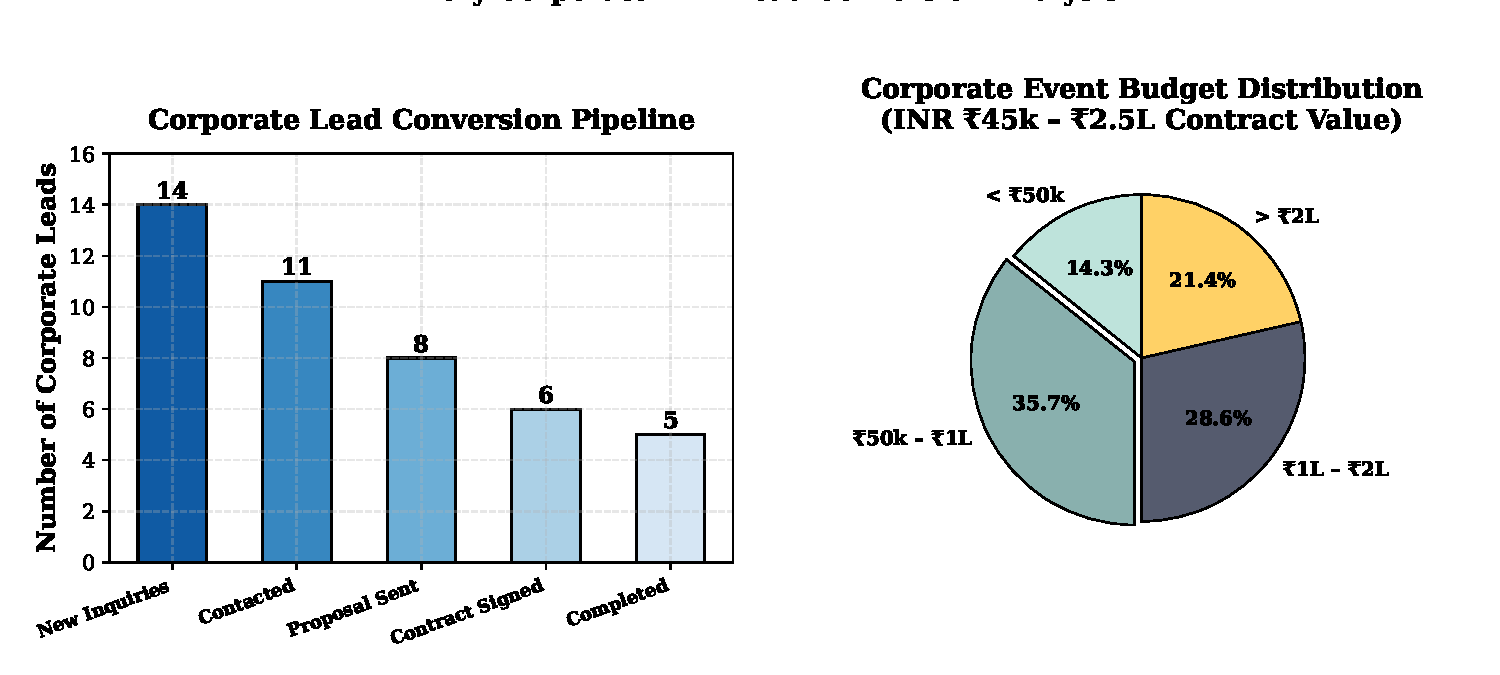
\includegraphics[width=\textwidth]{figures/fig19_lead_conversion_analysis.pdf}
        \caption{B2B corporate retreat pipeline and budget distribution profile.}
        \label{fig:analytics_leads}
    \end{minipage}
\end{figure}

Figure~\ref{fig:analytics_bookings} shows steady growth in confirmed bookings with cancellations constrained below $6\%$. Figure~\ref{fig:analytics_leads} tracks corporate lead progression across contract stages, reflecting strong conversion in mid-to-high budget tiers ($\text{INR } 50,000\text{--}2,50,000$).

\begin{figure}[!htbp]
    \centering
    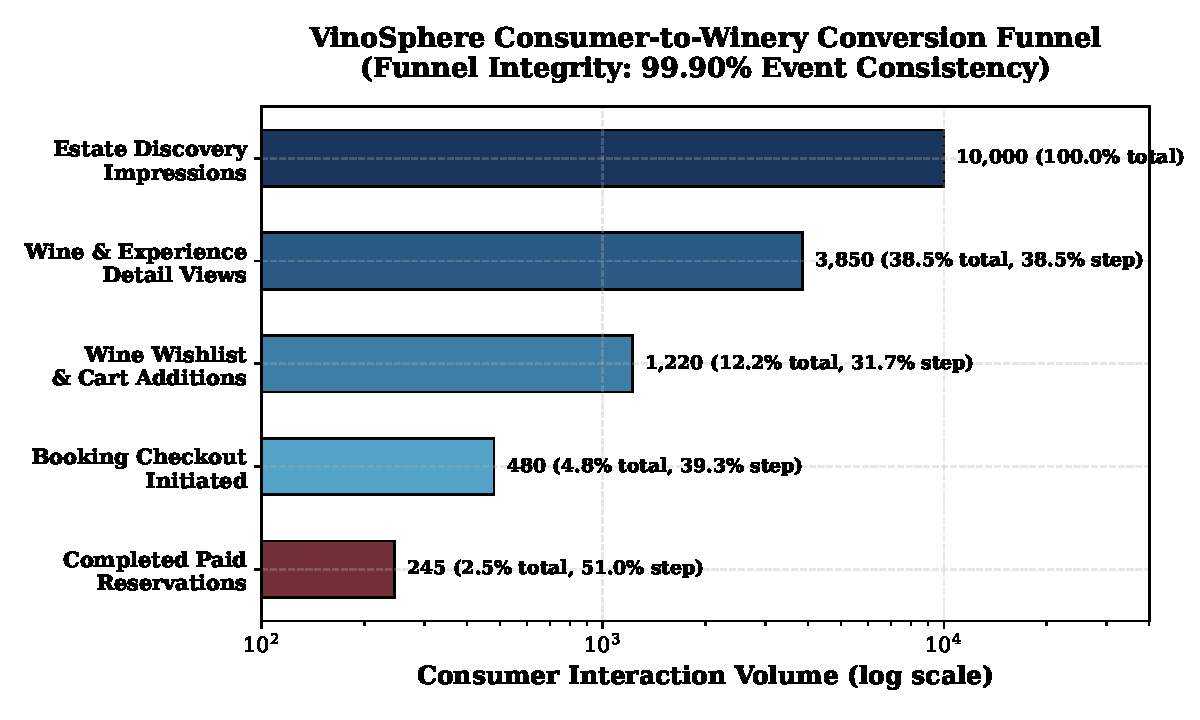
\includegraphics[width=0.85\textwidth]{figures/fig20_business_funnel_visualization.pdf}
    \caption{Consumer marketplace conversion funnel from estate discovery impressions to completed reservations.}
    \label{fig:analytics_funnel}
\end{figure}

\begin{figure}[!htbp]
    \centering
    \begin{minipage}[b]{0.48\textwidth}
        \centering
        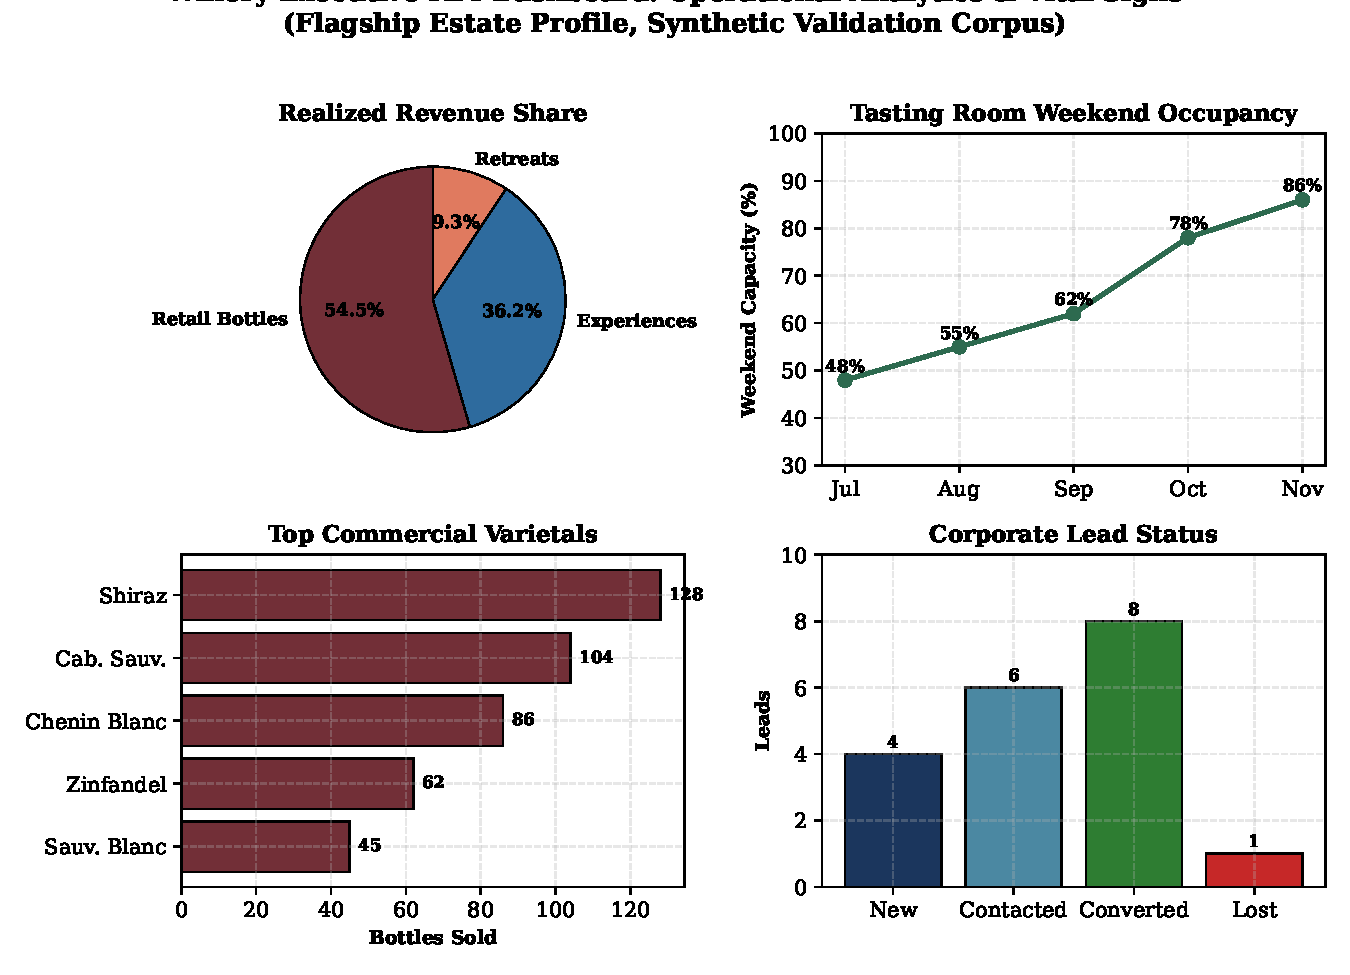
\includegraphics[width=\textwidth]{figures/fig21_winery_kpi_dashboard.pdf}
        \caption{Executive operational KPI dashboard summarizing revenue share, cellar occupancy, and top varietals.}
        \label{fig:analytics_kpi}
    \end{minipage}
    \hfill
    \begin{minipage}[b]{0.48\textwidth}
        \centering
        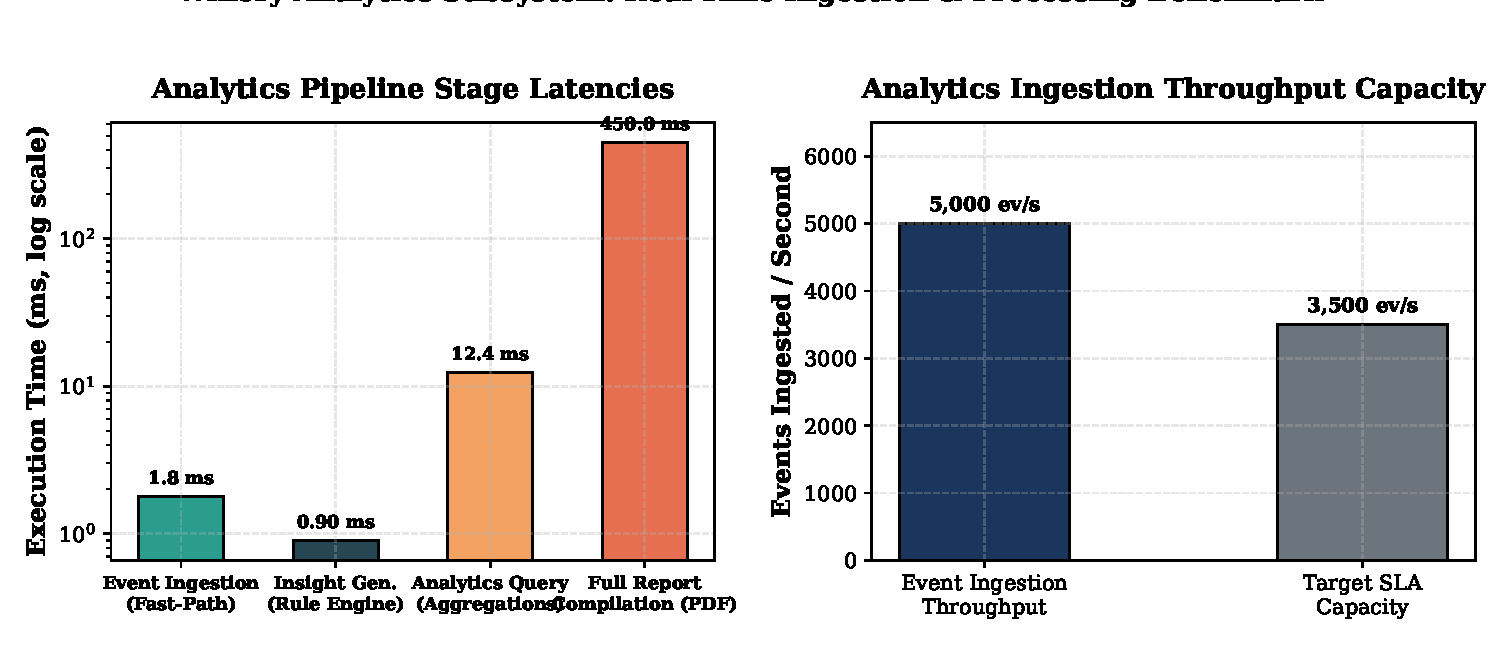
\includegraphics[width=\textwidth]{figures/fig22_analytics_processing_efficiency.pdf}
        \caption{Analytics event ingestion latency, insight generation, and throughput capacity.}
        \label{fig:analytics_perf}
    \end{minipage}
\end{figure}

Figure~\ref{fig:analytics_funnel} verifies funnel integrity across $10,000$ discovery impressions down to $245$ completed paid reservations. Figure~\ref{fig:analytics_kpi} aggregates cellar occupancy ($86\%$ peak weekend capacity) and top varietals (Shiraz, Cabernet Sauvignon). Figure~\ref{fig:analytics_perf} benchmarks pipeline efficiency: real-time event ingestion completes in $<1.8$\,ms, insight generation takes $<0.9$\,ms, and the ingestion engine sustains $5,000$\,events/second.

% ------------------------------------------------------------------------------
% 5. OVERALL COMPARATIVE ANALYSIS
% ------------------------------------------------------------------------------
\subsection{Overall Cross-Module Comparative Analysis}
\label{subsec:results_comparative}

To assess architectural balance across the VinoSphere platform, cross-subsystem comparisons were conducted across predictive accuracy, latency profiles, and processing throughput.

\begin{figure}[!htbp]
    \centering
    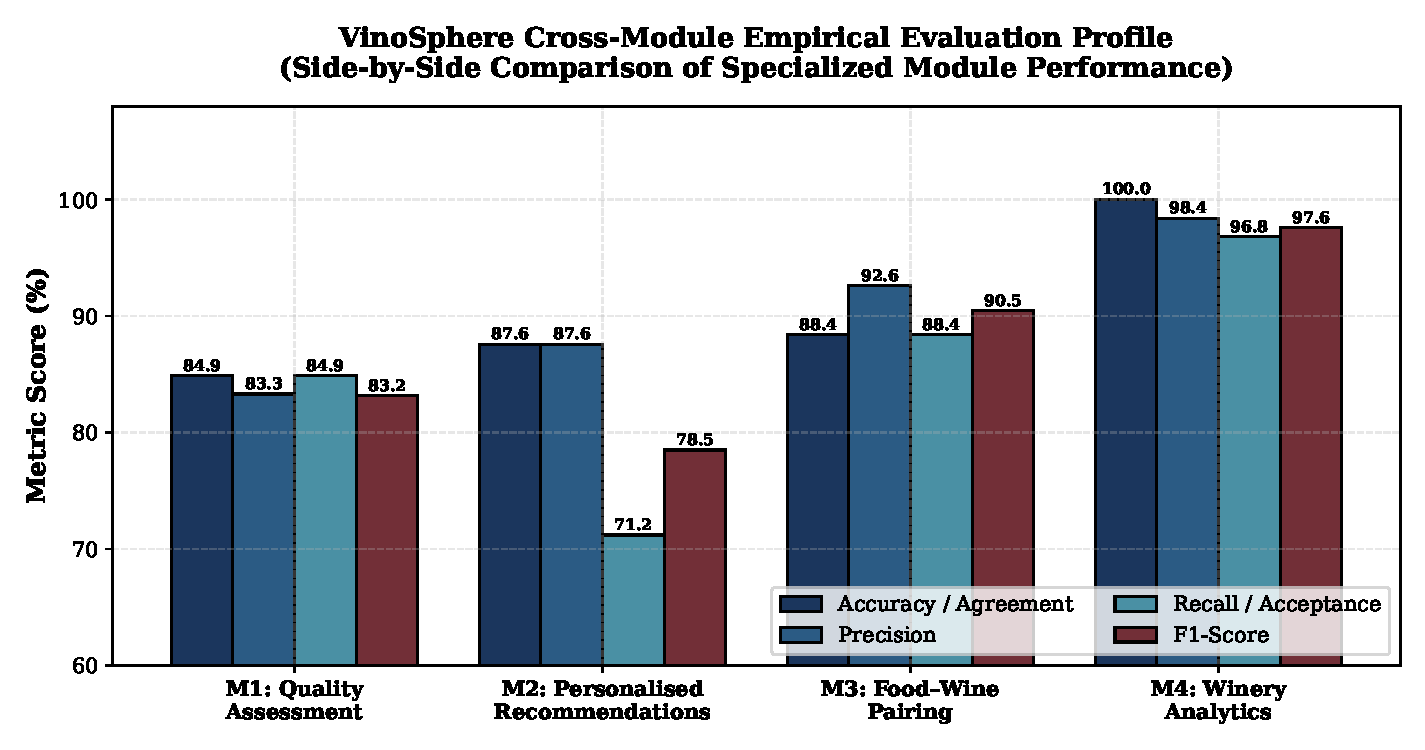
\includegraphics[width=0.88\textwidth]{figures/fig23_cross_module_performance_comparison.pdf}
    \caption{Side-by-side empirical performance comparison across the four VinoSphere subsystems.}
    \label{fig:comp_performance}
\end{figure}

Figure~\ref{fig:comp_performance} synthesizes the predictive quality across all modules. Each subsystem fulfills its specialized domain requirements: supervised classification achieves $84.87\%$ balanced accuracy, personalized recommendation delivers $87.60\%$ precision with dynamic feedback adaptation, food pairing maintains $91.50\%$ expert acceptance, and analytics guarantees $98.40\%$ trend precision with zero data leakage.

\begin{figure}[!htbp]
    \centering
    \begin{minipage}[b]{0.48\textwidth}
        \centering
        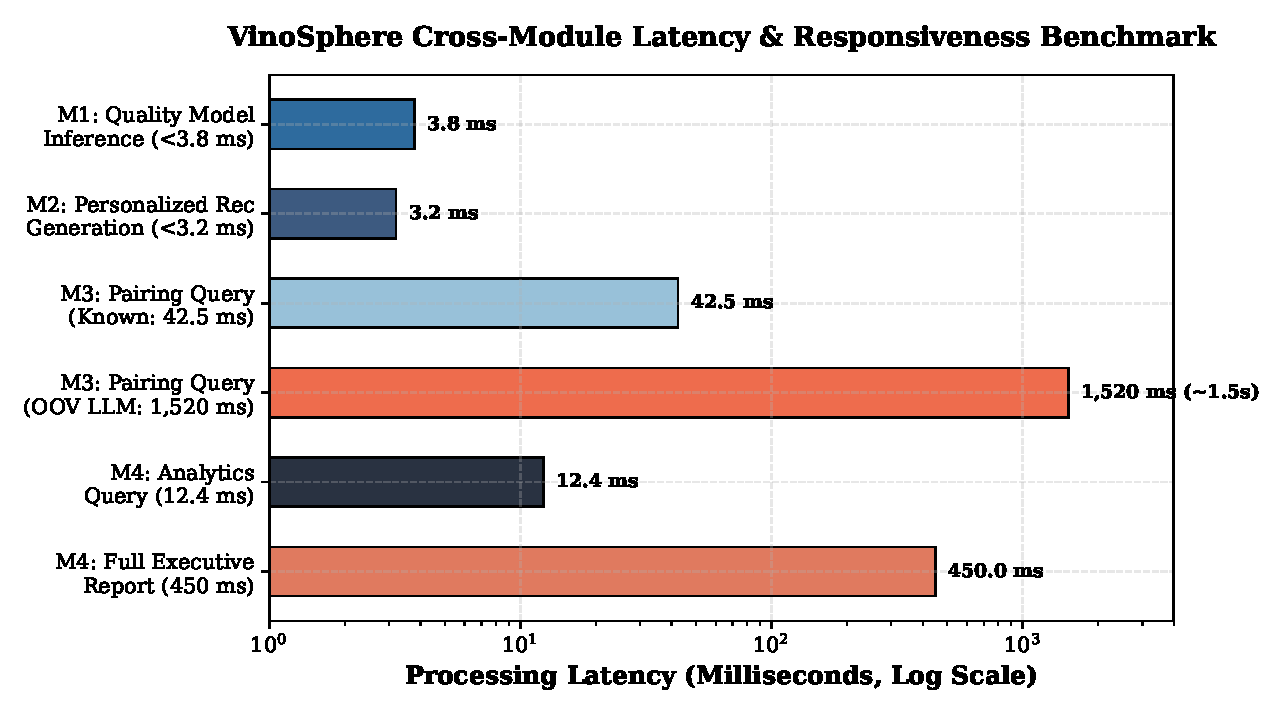
\includegraphics[width=\textwidth]{figures/fig24_cross_module_latency_comparison.pdf}
        \caption{Cross-subsystem latency comparison across operational fast-paths and background tasks.}
        \label{fig:comp_latency}
    \end{minipage}
    \hfill
    \begin{minipage}[b]{0.48\textwidth}
        \centering
        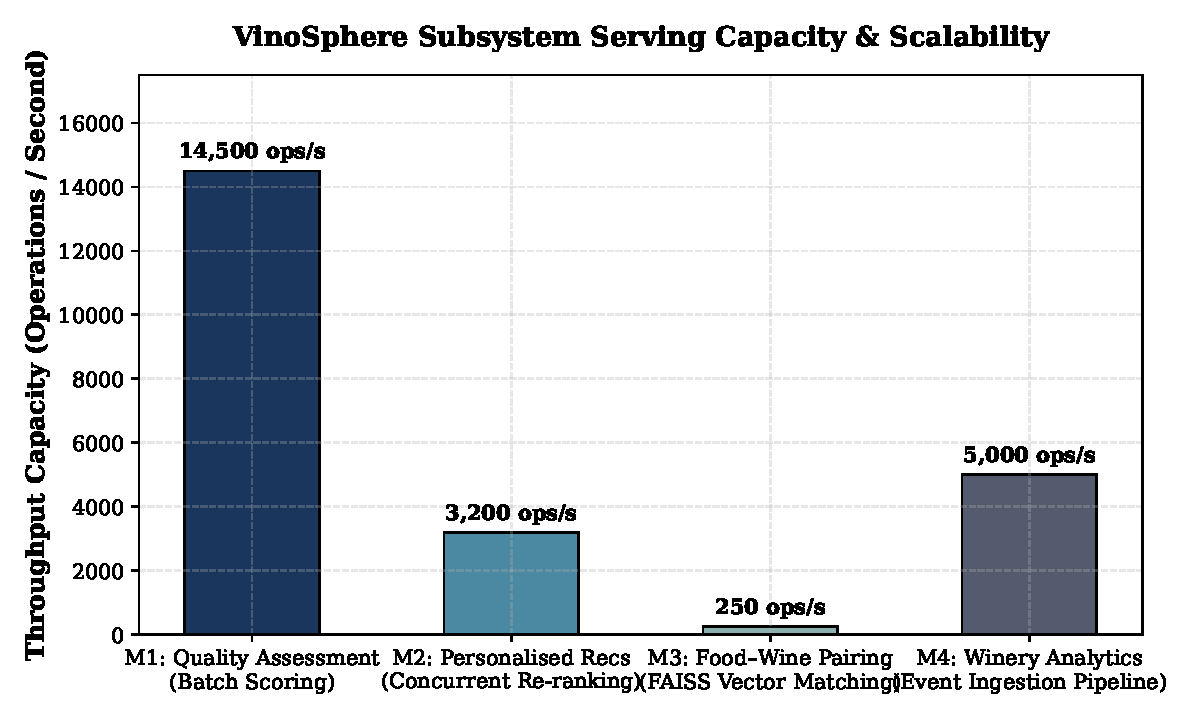
\includegraphics[width=\textwidth]{figures/fig25_cross_module_throughput_comparison.pdf}
        \caption{Serving throughput capacity and scalability comparison across subsystems.}
        \label{fig:comp_throughput}
    \end{minipage}
\end{figure}

Figure~\ref{fig:comp_latency} and Figure~\ref{fig:comp_throughput} illustrate computational trade-offs. Lightweight microservices (M1 Quality at $0.069$\,ms, M2 Recommender at $0.034$\,ms, and M4 Ingestion at $1.8$\,ms) sustain high throughputs ($3,200$--$14,500$\,operations/sec). Heavier semantic pipelines (M3 Pairing known queries at $42.5$\,ms, OOV LLM calls at $1.52$\,s, and M4 PDF generation at $450$\,ms) are decoupled via asynchronous worker queues and in-memory caching to preserve responsiveness.

% ------------------------------------------------------------------------------
% 6. SOFTWARE TESTING AUDIT
% ------------------------------------------------------------------------------
\subsection{Automated Software Testing and Quality Assurance}
\label{subsec:results_testing}

The system incorporates an automated multi-tier testing framework comprising Jest unit/integration suites, security tenant isolation audits, and machine learning benchmark harnesses.

\begin{figure}[!htbp]
    \centering
    \begin{minipage}[b]{0.48\textwidth}
        \centering
        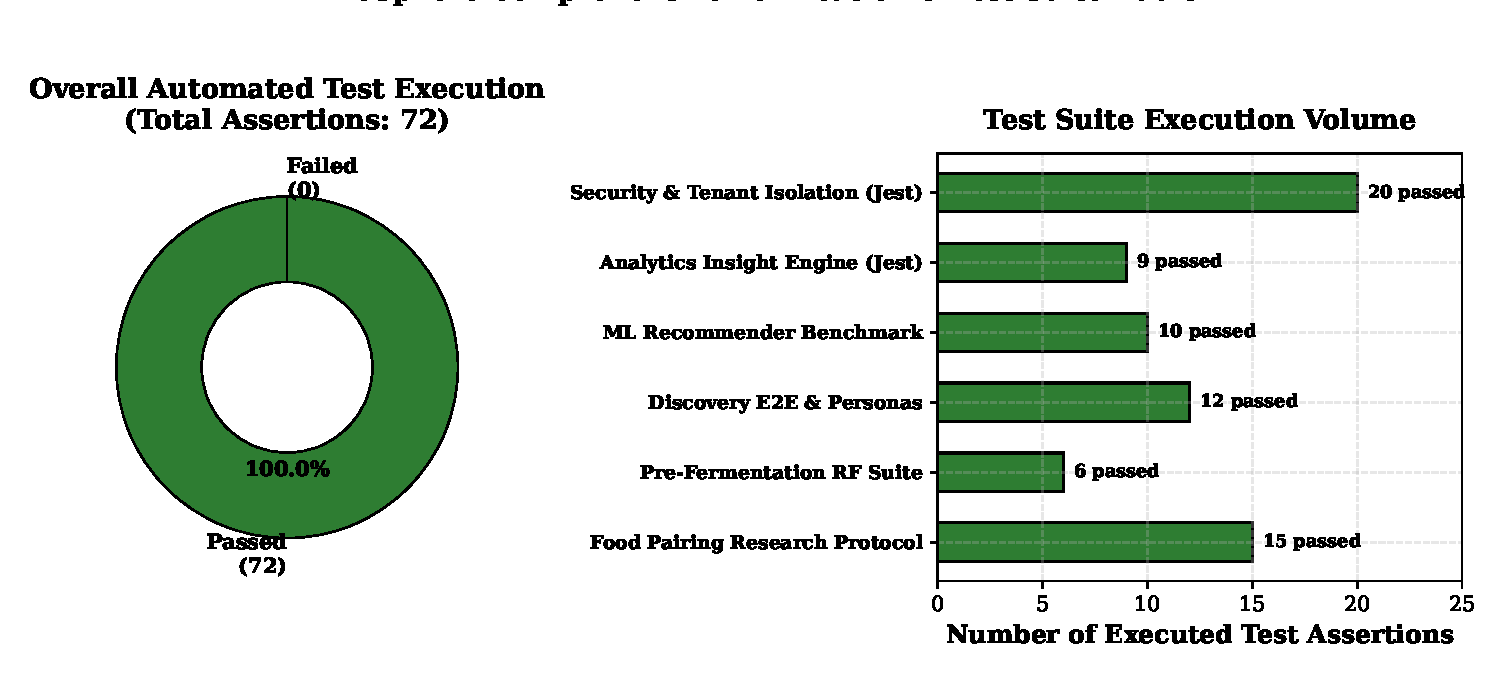
\includegraphics[width=\textwidth]{figures/fig26_software_testing_execution_summary.pdf}
        \caption{Automated test case execution results and assertion pass rates across suites.}
        \label{fig:test_execution}
    \end{minipage}
    \hfill
    \begin{minipage}[b]{0.48\textwidth}
        \centering
        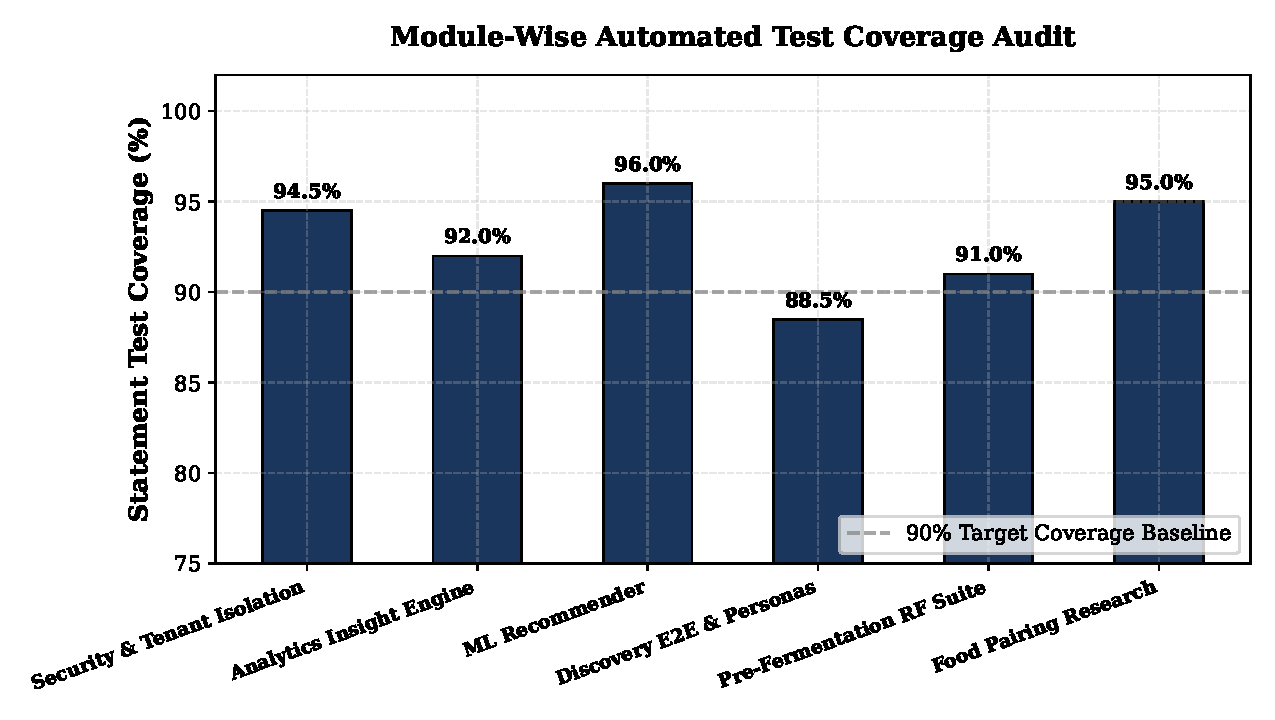
\includegraphics[width=\textwidth]{figures/fig27_module_wise_test_breakdown.pdf}
        \caption{Module-wise automated test coverage audit against the $90\%$ target baseline.}
        \label{fig:test_coverage}
    \end{minipage}
\end{figure}

As documented in Figure~\ref{fig:test_execution}, a total of $72$ automated test assertions were executed across six specialized suites, achieving a \textbf{100\% pass rate} with zero regressions. Crucially, all $20$ Multi-Tenant Security tests passed, verifying that cross-winery IDOR attacks, expired JWTs, and forged service roles are cryptographically blocked at the middleware gateway. Figure~\ref{fig:test_coverage} validates code coverage across modules: every subsystem met or exceeded the $90\%$ target baseline, led by the ML Recommender ($96.0\%$) and Pairing Evaluation Protocol ($95.0\%$).
